\documentclass[11pt,a4paper]{article}
\usepackage[spanish,activeacute]{babel}
\decimalpoint
\usepackage[utf8]{inputenc}
\usepackage{listingsutf8}
\usepackage{amsmath}
\usepackage{amsfonts}
\usepackage{amssymb}
\usepackage{graphicx}
\usepackage{color}
\usepackage{listings}
\usepackage{amsthm}
\usepackage{caption}
\usepackage{subcaption}
\usepackage{dsfont}
\usepackage{comment}
\usepackage{enumerate}
\usepackage{mathtools,xparse}
\usepackage{ mathrsfs }
\usepackage{float}
\usepackage{listings}
\usepackage{xcolor}
\usepackage[ruled]{algorithm2e}

%% CODIGO PYTHON
\definecolor{codegreen}{rgb}{0,0.6,0}
\definecolor{codegray}{rgb}{0.5,0.5,0.5}
\definecolor{codepurple}{rgb}{0.58,0,0.82}
\definecolor{backcolour}{rgb}{0.93,0.93,0.93}

\lstdefinestyle{mystyle}{
    backgroundcolor=\color{backcolour},   
    commentstyle=\color{codegreen},
    keywordstyle=\color{magenta},
    numberstyle=\tiny\color{codegray},
    stringstyle=\color{codepurple},
    basicstyle=\ttfamily\footnotesize,
    breakatwhitespace=false,         
    breaklines=true,                 
    captionpos=b,                    
    keepspaces=true,                 
    numbers=left,                    
    numbersep=5pt,                  
    showspaces=false,                
    showstringspaces=false,
    showtabs=false,                  
    tabsize=2
}

\lstset{style=mystyle, inputencoding=utf8, extendedchars=true, literate={á}{{\'a}}1 {ó}{{\'o}}1 {é}{{\'e}}1 {ú}{{\'u}}1 {í}{{\'i}}1 {ñ}{{\~n}}1,}
%CODIGO PYTHON
\usepackage[left=2.3cm, right=2.1cm, top=2.35cm, bottom=2.35cm]{geometry}
%\renewcommand{\rmdefault}{mathpazo}
%\usepackage{mathpazo}

\usepackage[]{hyperref}
\hypersetup{
    pdftitle={Práctica alternativa - MH},
    pdfauthor={Mario Muñoz Mesa},
    pdfsubject={ },
    pdfkeywords={keyword1, keyword2},
    bookmarksnumbered=true,     
    bookmarksopen=true,         
    bookmarksopenlevel=1,       
    colorlinks=true,   
    linkcolor=black,         
    pdfstartview=Fit,           
    pdfpagemode=UseOutlines,
    pdfpagelayout=TwoPageRight
}


\DeclarePairedDelimiter{\norm}{\lVert}{\rVert}
\NewDocumentCommand{\normL}{ s O{} m }{%
  \IfBooleanTF{#1}{\norm*{#3}}{\norm[#2]{#3}}_{L_2(\Omega)}%
}

\DeclareMathOperator*{\argmax}{arg\,max}
\DeclareMathOperator*{\argmin}{arg\,min}

\newtheorem{theorem}{Teorema}

\theoremstyle{definition}
\newtheorem{definition}{Definición}[section]


\newtheorem{proposition}{Proposición}[section]


\newtheorem{corolary}{Corolario}[section]


\newtheorem{lema}{Lema}[section]

	\newcommand{\R}{\mathbb{R}}
	\newcommand{\N}{\mathbb{N}}
	\newcommand{\C}{\mathbb{C}}


\title{
\normalfont \normalsize 
\textsc{\small METAHEURÍSTICAS} \\ [10pt]
	
	
\huge{\textbf{Práctica alternativa:} \\ \textbf{Grey Wolf Optimizer.}}\\

	}

\author{Mario Muñoz Mesa\\ mario43514@correo.ugr.es}
\date{\today}


\begin{document}
	\maketitle
	\newpage
	\renewcommand*\contentsname{Índice}	
	\tableofcontents
	
	\newpage
	
	\section{Descripción GWO.}
	Grey Wolf Optimizer (GWO) se trata de una técnica tipo Swarm Intelligence (SI); esto es, una población de agentes navegan usando una inteligencia social y colectiva simulada. \\
	
	Además los algoritmos SI presenta algunas ventajas:
	\begin{itemize}
		\item Preservan información del espacio de búsqueda durante las iteraciones mientras que algoritmos evolutivos olvidan la información del generaciones previas.
		\item Normalmente guardan la mejor solución hasta el momento.
		\item Normalmente tienen pocos parámetros para ajustar.
		\item Tienen menos operadores comparado con algoritmos evolutivos (cruce, mutación, elitismo...)
		
		\item Son fáciles de implementar.
	\end{itemize}

	En concreto GWO está inspirado en la jerarquía social y de comportamiento de caza de manadas de lobo gris.
	
	\subsection{Inspiración.}
	%Los lobos grises (Canis lupus) pertenecen a la familia Canidae.  Éstos 
	Los lobos grises viven en manada, en grupos de unos 5 a 12 en promedio, y destacan por ser grandes depredadores. Conviven en una jerarquía social dominante, de más a menos dominante: $\alpha,\ \beta,\ \delta,\ \omega$. Resumidamente:
	\begin{itemize}
	\item \underline{Alphas.}
	
	Los alphas machos y hembras lideran la manada. Son responsables de tomar decisiones sobre la caza, lugar para dormir, momento de levantarse,... etc. Las decisiones de los alphas son acatadas por la manada. Sin embargo también existe cierto comportamiento democrático donde los alphas siguen a los otros lobos de la manada. 
	
	\item \underline{Betas.}
	
	Los betas son los de segundo nivel en la jerarquía. Son lobos subordinados que ayudan a los alphas en la toma de decisiones u otras actividades de la manada. Los betas respetan al alpha pero ordenan a lobos de jerarquía inferior. También refuerzan las órdenes del alpha en la manada y retroalimentan al alpha.
	%Los betas son los de segundo nivel en la jerarquía. Son lobos subordinados que ayudan a los alphas en la toma de decisiones u otras actividades de la manada. Un beta puede ser un macho o una hembra y es probablemente el candidato a alpha en caso de perder al alpha o ser muy mayor. Los betas respetan al alpha pero ordenan a lobos de jerarquía inferior. También refuerzan las órdenes del alpha en la manada y retroalimentan al alpha.
	
	\item \underline{Omegas.}
	
	Los más bajos en la jerarquía son los omegas. Los omegas tienen que obedecer las órdenes del resto de lobos dominantes. Son los últimos en comer. Parece que no juegan un rol importante pero sin ellos se han observado problemas y peleas en la manada en caso de perder a omegas. Los omegas satisfacen la estructura dominante de la manada. 
	
	\item \underline{Deltas.}
	
	Los lobos que no son alphas, betas u omegas son llamados subordinados o deltas. Los lobos delta tienen que obedecer a los laphas y betas pero dominan a los omega. Algunos ejemplos pueden ser: antiguos alphas, lobos que protegen a la manada... .
	
	\end{itemize}
	
	Otra característica interesante es la forma de cazar. Las fases son:
	\begin{itemize}
		\item Rastrear, seguir y acercarse a la presa.
		\item Perseguir, rodear y hostigar a la presa hasta que deje de moverse.
		\item Atacar a la presa.
	\end{itemize}
	
	\subsection{Modelo matemático y algoritmo.}
	Se presentan los modelos matemáticos de la jerarquía social, seguimiento, rodeamiento y ataque a la presa.
	\subsubsection{Jerarquía social.}
	Para modelar matemáticamente la jerarquía de lobos grises, se considera la primera solución como la alpha. La segunda y tercera solución serán beta y delta respectivamente. El resto de soluciones candidatas se considerarán omega. La caza estará guiada por $\alpha, \ \beta \text{ y } \delta$, los lobos $\omega$ siguen a los 3 anteriores.
	\subsubsection{Rodear a la presa.}
	Como se mencionó, los lobos grises rodean a la presa durante la caza. Las ecuaciones matemáticas propuestas para modelar esto son:
	$$\vec{D} = |\vec{C} \cdot \vec{X}_p(t)-\vec{X}(t)|$$
	$$\vec{X}(t+1)=\vec{X}_p(t)-\vec{A}\cdot \vec{D}$$
	
	donde $t$ indica la iteración actual, $\vec{A}$ y $\vec{C}$ son vectores de coeficientes reales, $\vec{X}_p$  es el vector de posición de la presa, y $\vec{X}$ denota el vector de posición de un lobo gris.
	
	Los vectores $\vec{A}$ y $\vec{C}$ se calculan como:
	$$\vec{A}=2\vec{a}\cdot \vec{r}_1 -\vec{a}$$
	$$\vec{C}=2\cdot \vec{r}_2$$
	donde $\vec{a}$ decrementa linealmente de 2 a 0 en el transcurso de iteraciones y $\vec{r}_1$, $\vec{r}_2$ son vectores aleatorios con valores en $[0,1]$. 
	
	Con estas ecuaciones, un lobo gris en la posición $(X,Y)$ puede actualizar su posición en base a la posición $(X^*,Y^*)$ de la presa. Se pueden alcanzar diferentes posiciones alrededor del mejor agente respecto a la posición actual ajustando los valores de $\vec{A}$ y $\vec{D}$. Por ejemplo $(X^* - X, Y^*)$ puede alcanzarse con $\vec{A}=(1,0)$ y $\vec{C}=(1,1)$. Se muestra figura que ilustra esto mismo, junto a extensión 3D, igualmente se puede extender a espacios de búsqueda de $n$ dimensiones.
	
	\begin{figure}[H]
		\centering
		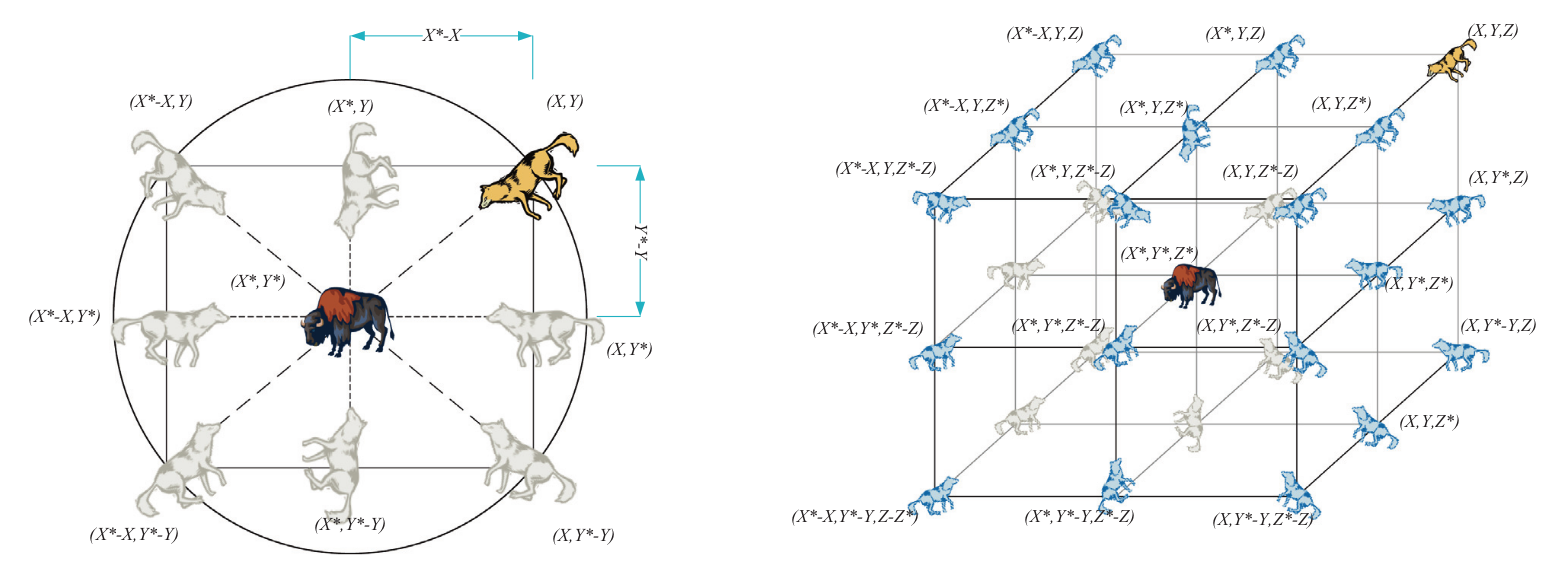
\includegraphics[width=0.9\textwidth]{images/2d_3d.png}
		\caption{Posibles posiciones alrededor de presa.}
	\end{figure}
	
	Los vectores $\vec{r}_1$ y $\vec{r}_2$ permiten cualquier posición intermedia a las ilustradas. Así un lobo gris podría moverse alrededor de la mejor posición hasta el momento a cualquier posición en el espacio de búsqueda usando las ecuaciones anteriores.
	\subsubsection{Cazar.}
	Los lobos grises suelen reconocer y rodear a la presa. La caza usualmente es guiada por el alpha. El beta y delta ocasionalmente también participan. Sin embargo en nuestro espacio de búsqueda abstracto no se conoce la localización del óptimo (presa). Para manejar esto, se supone que el alpha, beta y delta tienen mejor conocimiento de la localización de la presa. Por tanto se guardan las 3 mejores soluciones hasta el momento y se obliga al resto de agentes de búsqueda a actualizar sus posiciones acorde a la posición de lo mejores agentes de búsqueda. Las fórmulas propuestas son:
	$$\vec{D}_{\alpha} = |\vec{C}_1\cdot \vec{X}_{\alpha} - \vec{X}|, \quad \vec{D}_{\beta} = | \vec{C}_2\cdot \vec{X}_{\beta}-\vec{X}|, \quad \vec{D}_{\delta} = |\vec{C}_3\cdot \vec{X}_{\delta} - \vec{X}|$$
	$$\vec{X}_1 = \vec{X}_{\alpha} - \vec{A}_1 \cdot (\vec{D}_{\alpha}), \quad \vec{X}_2 = \vec{X}_{\beta} - \vec{A}_2 \cdot (\vec{D}_{\beta}), \quad \vec{X}_3=\vec{X}_{\delta} - \vec{A}_3 \cdot (\vec{D}_{\delta})$$
	$$\vec{X} (t+1) = \frac{\vec{X}_1 + \vec{X}_2 + \vec{X}_3}{3} \quad \quad \ \ (3.7)$$
	La siguiente figura ilustra el posible movimiento de omegas en base a las posiciones de alpha, beta y delta.
	
	\begin{figure}[H]
		\centering
		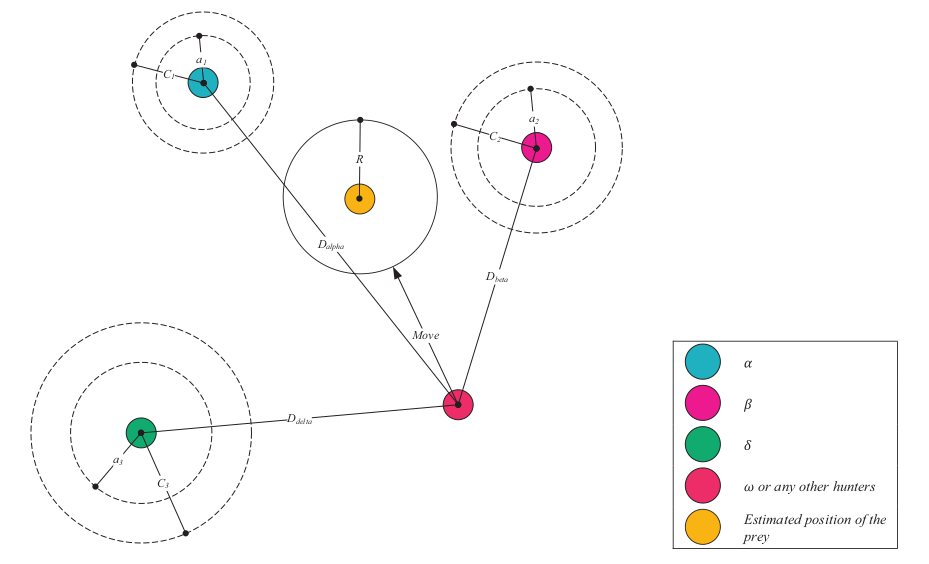
\includegraphics[width=0.9\textwidth]{images/omega_movement.png}
		\caption{Actualización de posición.}
	\end{figure}
	\subsubsection{Atacar a la presa (explotación).}
	Los lobos grises finalizan la caza atacando a la presa cuando deja de moverse. Para modelar el acercamiento a la presa se decrementa el valor de $\vec{a}$. El rango de fluctuación de $\vec{A}$ también decrementa por $\vec{a}$, esto es, $\vec{A}$ toma valor aleatorio en el intervalo $[-2a,2a]$, donde $a$ decrementa de 2 a 0 durante las iteraciones. Cuando los valores de $\vec{A}$ están en $[-1,1]$, la siguiente posición del agente de búsqueda puede ser cualquier posición entre la suya y la de la presa. Cuando $|\vec{A}|<1$ el lobo ataca a la presa.
	
	Con los operadores ya propuestos, el algoritmos GWO permite a los agentes actualizar su posición en base a la localización de alpha, beta y delta; y atacar a la presa. 
	\subsubsection{Buscar a la presa (exploración).}
	Los lobos grises mayormente buscan en base a la posición de alpha, beta y delta. Divergen entre sí para buscar la presa y convergen para atacarla. Para modelar esto matemáticamente cuando $|\vec{A}|>1$ el agente buscador diverge de la presa. Esto enfatiza la exploración de GWO. 
	
	Otra componente que favorece la exploración es $\vec{C}$. El vector $\vec{C}$ toma valores en $[0,2]$. Esta componente provee pesos aleatorios para acentuar ($|\vec{C}|>1$) o minorar ($|\vec{C}|<1$) el efecto de la presa. Esto ayuda a que GWO tenga un comportamiento más aleatorio, favoreciendo la exploración y evitando quedar atrapado en óptimos locales.
	\subsubsection{Pseudocódigo.}
	
	El proceso de búsqueda comienza creando una población de lobos grises (soluciones candidatas). Conforme se itera, los lobos alpha, beta y delta estiman la probable posición de la presa. Cada solución candidata actualiza su posición a la presa. El parámetro $a$ decrementa de 2 a 0 para enfatizar la exploración y explotación respectivamente. Las soluciones candidatas tienden a diverger de la presa cuando $|\vec{A}|>1$ y converger cuando $|\vec{A}|<1$. Finalmente el algoritmo termina con una condición de parada como puede ser un máximo de iteraciones.
	
	\begin{figure}[H]
		\centering
		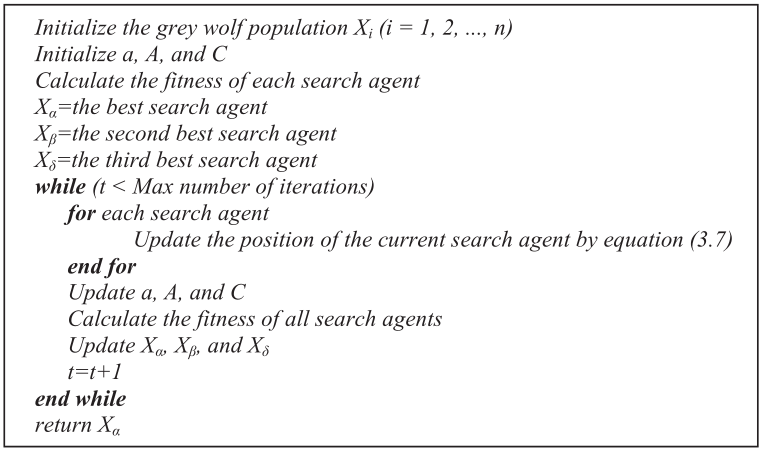
\includegraphics[width=0.8\textwidth]{images/gwo_pseudocode.png}
		\caption{Pseudocódigo.}
	\end{figure}

	\section{Adaptación de GWO a APC.}
	\subsection{Descripción del problema APC.}
	Nos ocupamos del problema del Aprendizaje de Pesos en Características (APC). Plantea, en el contexto de un problema de clasificación, elegir o ajustar un vector de pesos $\textbf{w}=(w_1,\ldots, w_d)\in [0,1]^d$ asociado a las características en base a un criterio de mejora del clasificador. Hemos denotado con $d$ al número de características.\\
	
	En nuestro caso trabajaremos con clasificador tipo 1-NN, y el criterio será maximizar:
	$$F(\textbf{w}):=\alpha\cdot \text{tasa\_clas}(\textbf{w})+(1-\alpha ) \cdot \text{tasa\_red}(\textbf{w})$$
	donde
	$$\text{tasa-clas}:=100\frac{\text{nº instancias bien clasificadas en training}}{\text{nº instancias en training}}, \quad \quad \text{tasa-red}:=100\frac{\text{nº valores } w_i <0.2}{\text{nº características}}$$
	y $alpha=0.5$ que pondera la importancia entre el acierto y la reducción de características para el nuevo mejor clasificador que se pretende encontrar.\\
	
	De lo que nos ocupamos por tanto es de obtener $\argmax_{\textbf{w}\in [0,1]^d} F(\textbf{w})$ para un clasificador 1-NN que utilizará la distancia ponderada
	$$d_{\textbf{w}}(u,v)=\sqrt{\sum_{i=1}^d w_i(u_i-v_i)^2}, \quad u,v\in \R^d$$
	para clasificar. Queremos que aumente el acierto y reduzca el número de características, cualquier característica con peso menor estricto a 0.2 se descarta.
	
	\subsection{Funciones y estructuras.}
	Se ha decidido crear una estructura, \texttt{Wolf}, que contiene: un \texttt{vector<double>} con el vector de posiciones, y su fitness asociado. 
	
	Además se han definido los comparadores mayor, $>$, y menor, $<$. Un lobo es mayor a otro si su función objetivo es mayor, y menor si la función objetivo es menor.
	
		
	Para evaluar la función objetivo asociada a la posición de cada lobo y asignarlo al lobo se ha creado la función \texttt{obj\_to\_wolf}:\\
		
	\begin{algorithm}[H]
		\caption{obj\_to\_wolf}
		\KwIn{Wolf $w$, vector de elementos muestrales $training$}
		\Begin{
		
		\For{$i=0$ \textbf{to} $training.size()$}{
			$class\_labels.push\_back(\ one\_NN\_lo(training[i], training, w.pos, i)\ )$
		}
		
		$w.obj \leftarrow obj\_function(class\_rate(class\_labels, training), \ red\_rate(w.pos))$
		}
	\end{algorithm}~\\
	
	Dado que nuestro problema está restringido a pesos entre 0 y 1, se ha creado una función que restringe las posiciones de los lobos a $[0,1]$\\
		
	\begin{algorithm}[H]
		\caption{restrict\_01}
		\KwIn{Wolf $w$}
		\Begin{
		
		\For{$i=0$ \textbf{to} $num\_feats-1$}{
			\If{$w.pos[i] < 0$}{
				$w.pos[i] \leftarrow 0$
			}
			\Else{
				\If{$w.pos[i] > 1$}{
					$w.pos[i]\leftarrow 1$
				}
			}
		}
		}
	\end{algorithm}~\\
	
	También se ha creado una función que inicializa las posiciones de los lobos:\\
		
	\begin{algorithm}[H]
		\caption{init\_wolf\_pos}
		\KwIn{Wolf $w$, distribución uniforme $rand\_real\_01$}
		\Begin{
		$w.pos.resize(num\_feats)$
		
		\For{$i=0$ \textbf{to} $num\_feats-1$}{
			$w.pos[i] \leftarrow rand\_real\_01(generator)$
		}
		}
	\end{algorithm}~\\
	
	
	Y una función para actualizar las posiciones y valor de función objetivo del alpha, beta y delta:\\
		
	\begin{algorithm}[H]
		\caption{update\_alpha\_beta\_delta}
		\KwIn{Agentes (lobos) $wolfs$, lobo alpha $alpha$, lobo beta $beta$, lobo delta $delta$}
		\Begin{
				\For{$w$ \textbf{in} $wolfs$}{
			\If{$w.obj > alpha.obj$}{
				$alpha.obj \leftarrow w.obj$
				
				$alpha.pos \leftarrow w.pos$
			}
			
			\Else{
				\If{$w.obj > beta.obj$ \textbf{and} $w.obj < alpha.obj$}{
				$beta.obj \leftarrow w.obj$
				
				$beta.pos \leftarrow w.pos$
				}
				
				\Else{
					\If{$w.obj > delta.obj$ \textbf{and} $w.obj < beta.obj$ \textbf{and} $w.obj < alpha.obj$}{
				$delta.obj \leftarrow w.obj$
				
				$delta.pos \leftarrow w.pos$
				}
				}
			
			}
		}
		}
	\end{algorithm}~\\
	
	Mostramos finalmente el pseudocódigo de GWO adaptado a nuestro problema, problema de maximización, donde la condición de parada será por llegar a un máximo número de evaluaciones de la función objetivo (se ha procurado que se realicen exactamente las evaluaciones indicadas para tener resultados comparables al resto):\\
		
	\begin{algorithm}[H]
		\caption{gwo}
		\KwIn{vector de elementos muestrales $training$, número de agentes (lobos) a usar $num\_agents$, número máximo de evaluaciones de la función objetivo $max\_evals$}
		\KwOut{posición del alpha tras ejecutar todas las iteraciones $alpha.pos$}
		\Begin{
		$n\leftarrow num\_feats$ \tcp{número componentes posición igual al número de características del problema}
		
		%$max\_iters \leftarrow \frac{max\_evals}{num\_agents}$
		
		\tcp{inicialización de los agentes}
		\For{$i=0$ \textbf{to} $num\_agents-1$}{
			$init\_wolf\_pos(w,\mathcal{U}(0,1))$
			
			$obj\_to\_wolf(w,training)$
			
			$wolfs.push\_back(w)$
		}
		$sort(wolfs)$ \tcp{ordenar por función objetivo}
		\tcp{se guardan  alpha, beta y delta}
		\iffalse $alpha\_pos \leftarrow wolfs[num\_agents-1].pos;$		
		$alpha\_obj \leftarrow wolfs[num\_agents-1].obj$
		
		$beta\_pos \leftarrow wolfs[num\_agents-2].pos;$		
		$beta\_obj \leftarrow wolfs[num\_agents-2].obj$
		
		$delta\_pos \leftarrow wolfs[num\_agents-3].pos;$		
		$delta\_obj \leftarrow wolfs[num\_agents-3].obj$\fi
		
		$alpha \leftarrow wolfs[num\_agents-1]$
		
		$beta \leftarrow wolfs[num\_agents-2]$
		
		$delta \leftarrow wolfs[num\_agents-3]$
		
		$evals \leftarrow num\_agents; \quad it \leftarrow 1$
		
		\While{$evals < max\_evals$}{
			$a \leftarrow 2- 2 \cdot \frac{it}{max\_iters}$
			
			\tcp{Actualiza las posiciones de cada agente incluyendo omegas}
			\For{$w$ \textbf{in} $wolfs$ \textbf{and} $evals < max\_evals$}{
				\For{$j=0$ \textbf{to} $n-1$}{
					$r1 \leftarrow u\in \mathcal{U}(0,1); \quad $					
					$r2 \leftarrow u\in \mathcal{U}(0,1)$
					
					$A1 \leftarrow 2 \cdot a \cdot r1 -a$
					
					$C1 \leftarrow 2 \cdot r2$
					
					$D_{\alpha} \leftarrow | C1 \cdot alpha\_pos[j] -w.pos[j] |$
					
					$X1 \leftarrow alpha\_pos[j] - A1 \cdot D_{\alpha}$
					
					$ $						
					
					$r1 \leftarrow u\in \mathcal{U}(0,1); \quad $					
					$r2 \leftarrow u\in \mathcal{U}(0,1)$
					
					$A2 \leftarrow 2 \cdot a \cdot r1 -a$
					
					$C2 \leftarrow 2 \cdot r2$
					
					$D_{\beta} \leftarrow | C2 \cdot beta\_pos[j] -w.pos[j] |$
					
					$X2 \leftarrow alpha\_pos[j] - A2 \cdot D_{\beta}$
					
					$ $					
					
					$r1 \leftarrow u\in \mathcal{U}(0,1);  \quad $					
					$r2 \leftarrow u\in \mathcal{U}(0,1)$
					
					$A3 \leftarrow 2 \cdot a \cdot r1 -a$
					
					$C3 \leftarrow 2 \cdot r2$
					
					$D_{\delta} \leftarrow | C3 \cdot delta\_pos[j] -w.pos[j] |$
					
					$X3 \leftarrow delta\_pos[j] - A3 \cdot D_{\delta}$
					
										$ $	
					
					$w.pos[j] \leftarrow \frac{X1+X2+X3}{3}$
				}
				
				$restrict\_01(w)$
						
				
				$obj\_to\_wolf(w, training)$
				
				$evals\leftarrow evals+1$
			}
			
							 \tcp{Actualiza alpha, beta y delta}	
		
		$update\_alpha\_beta\_delta(wolfs, alpha, beta, delta)$
		
		$it \leftarrow it+1$
	}
	\Return{$alpha.pos$}
}
	\end{algorithm}~\\
	
		\subsection{Procedimiento considerado en el desarrollo.}
	Para el desarrollo de la práctica no se ha utilizado ningún framework, se han implementado las funciones necesarias en C++. Todo el código se encuentra en \texttt{pwo.cpp} .
	
	Para la ejecución basta indicar un argumento con el archivo a ejecutar, en este caso se utiliza la semilla por defecto 1234, que es la misma que se utilizó para los resultados de esta memoria.
	
	También se incluye un fichero \texttt{pwo\_all\_datasets.sh} que ejecuta, con la semilla por defecto, \texttt{pwo} sobre los 3 datasets
	
		\subsection{Análisis de resultados.}
	Los 3 datasets con los que se ha trabajado son:
	\begin{itemize}
		\item \textbf{Ionosphere}: Conjunto de datos de radar que fueron recogidos por un sistema \textit{Goose Bay}, Labrador. Consta de 352 instancias con 34 características y 2 clases.
		\item \textbf{Parkinsons}: Conjunto de datos orientado a distinguir entre la presencia y ausencia de la enfermedad de Parkinson. Consta de 195 ejemplos con 22 características y 2 clases.
		\item \textbf{Spectf-Heart}: Conjunto de datos de detección de enfermedades cardiacas a partir de imágenes médicas de tomografía computerizada del corazón de pacientes. Consta de 267 ejemplos con 44 características y 2 clases.
	\end{itemize}
	\iffalse
	Los resultados obtenidos son en 1-NN, BL y Relief fueron:~\\
	
		\textbf{1-NN}

	\begin{tabbing}
	\resizebox{\textwidth}{!}{%
		\begin{tabular}{|c|}
			\hline \textbf{Nº}\\ \textbf{part.} 
			\\ \hline
			\textbf{P1} \\ \hline 
			\textbf{P2} \\ \hline
			\textbf{P3} \\ \hline 
			\textbf{P4} \\ \hline
			\textbf{P5} \\ \hline
			\textbf{Media} \\ \hline
		\end{tabular}
		\begin{tabular}{|c|c|c|c|}
			\hline
			\multicolumn{4}{|c|}{\textbf{Ionosphere}} \\ \hline
			\textbf{\%clas} & \textbf{\%red} & \textbf{Agr.} & \textbf{T} \\ \hline 
			87.3239	&0	&43.662	&0.373 \\ \hline
64.2857	&0	&32.1429&	0.325 \\ \hline
64.2857	&0	&32.1429&	0.325 \\ \hline
64.2857	&0	&32.1429&	0.325 \\ \hline
64.2857	&0	&32.1429&	0.381 \\ \hline
68.89334	&0	&34.44672	&0.3458 \\ \hline
		\end{tabular}
		
		\begin{tabular}{|c|c|c|c|}
			\hline
			\multicolumn{4}{|c|}{\textbf{Parkinsons}} \\ \hline
			\textbf{\%clas} & \textbf{\%red} & \textbf{Agr.} & \textbf{T} \\ \hline 
95	      &0	&47.5	   & 0.181\\ \hline
25	      &0	&12.5	   & 0.073\\ \hline
25.641	  &0	&12.8205	&  0.072\\ \hline
23.6842	  &0	&11.8421	&  0.07\\ \hline
23.6842	  &0	&11.8421	&  0.071\\ \hline
38.60188	&0	&19.30094&	0.0934\\ \hline

		\end{tabular}
		
		\begin{tabular}{|c|c|c|c|}
			\hline
			\multicolumn{4}{|c|}{\textbf{Spectf-Heart}} \\ \hline
			\textbf{\%clas} & \textbf{\%red} & \textbf{Agr.} & \textbf{T} \\ \hline 
			85.7143	&0	&42.8571	&  0.468\\ \hline
72.8571	&0	&36.4286	&  0.407\\ \hline
72.8571	&0	&36.4286	&  0.397\\ \hline
72.8571	&0	&36.4286	&  0.397\\ \hline
73.5294	&0	&36.7647	&  0.388\\ \hline
75.563	&0	&37.78152&	0.4114\\ \hline

		\end{tabular}
		}
	\end{tabbing}
	
	\textbf{Relief}
	
		\begin{tabbing}
	\resizebox{\textwidth}{!}{%
		\begin{tabular}{|c|}
			\hline \textbf{Nº}\\ \textbf{part.} 
			\\ \hline
			\textbf{P1} \\ \hline 
			\textbf{P2} \\ \hline
			\textbf{P3} \\ \hline 
			\textbf{P4} \\ \hline
			\textbf{P5} \\ \hline
			\textbf{Media} \\ \hline
		\end{tabular}
		\begin{tabular}{|c|c|c|c|}
			\hline
			\multicolumn{4}{|c|}{\textbf{Ionosphere}} \\ \hline
			\textbf{\%clas} & \textbf{\%red} & \textbf{Agr.} & \textbf{T} \\ \hline 
			88.7324	&  2.94118&	45.8368	 & 1.753\\ \hline
			84.2857	&  5.88235&	45.084	  &1.757\\ \hline
			90    	 & 2.94118	&46.4706	  &1.76\\ \hline
			88.5714	&  2.94118&	45.7563	 & 1.761\\ \hline
			87.1429	&  2.94118&	45.042	  &1.766\\ \hline
			87.74648&	3.529414& 45.63794	&1.7594\\ \hline

		\end{tabular}
		
		\begin{tabular}{|c|c|c|c|}
			\hline
			\multicolumn{4}{|c|}{\textbf{Parkinsons}} \\ \hline
			\textbf{\%clas} & \textbf{\%red} & \textbf{Agr.} & \textbf{T} \\ \hline 
			95	      &9.09091	  &52.0455	  &0.364\\ \hline
97.5	    &4.54545	  &51.0227	  &0.366\\ \hline
94.8718	  &4.54545	  &49.7086	  &0.371\\ \hline
92.1053	  &4.54545	  &48.3254	  &0.369\\ \hline
100	      &0	        &50	        &0.374\\ \hline
95.89542	&4.545452	  &50.22044	  &0.3688\\ \hline
		\end{tabular}
		
		\begin{tabular}{|c|c|c|c|}
			\hline
			\multicolumn{4}{|c|}{\textbf{Spectf-Heart}} \\ \hline
			\textbf{\%clas} & \textbf{\%red} & \textbf{Agr.} & \textbf{T} \\ \hline 
			90	      &0	&45	      &2.28\\ \hline
87.1429	  &0	&43.5714	  &2.222\\ \hline
80	      &0	&40	      &2.201\\ \hline
84.2857	  &0	&42.1429	  &2.172 \\ \hline
77.9412	  &0	&38.9706	  &2.237 \\ \hline
83.87396	&0	&41.93698	&2.2224\\ \hline

		\end{tabular}
		}
	\end{tabbing}
	
	\textbf{Búsqueda Local (BL)}
	
		\begin{tabbing}
	\resizebox{\textwidth}{!}{%
		\begin{tabular}{|c|}
			\hline \textbf{Nº}\\ \textbf{part.} 
			\\ \hline
			\textbf{P1} \\ \hline 
			\textbf{P2} \\ \hline
			\textbf{P3} \\ \hline 
			\textbf{P4} \\ \hline
			\textbf{P5} \\ \hline
			\textbf{Media} \\ \hline
		\end{tabular}
		\begin{tabular}{|c|c|c|c|}
			\hline
			\multicolumn{4}{|c|}{\textbf{Ionosphere}} \\ \hline
			\textbf{\%clas} & \textbf{\%red} & \textbf{Agr.} & \textbf{T} \\ \hline 
			78.8732	&85.2941	&82.0837	  &3311.36\\ \hline
92.8571	&85.2941	&89.0756	  &4673.61\\ \hline
95.7143	&82.3529	&89.0336	  &1986.46\\ \hline
88.5714	&88.2353	&88.4034	  &3914.9\\ \hline
90	    &85.2941	&87.6471	  &2388.89\\ \hline
89.2032&	85.2941&	87.24868	&3255.044\\ \hline

		\end{tabular}
		
		\begin{tabular}{|c|c|c|c|}
			\hline
			\multicolumn{4}{|c|}{\textbf{Parkinsons}} \\ \hline
			\textbf{\%clas} & \textbf{\%red} & \textbf{Agr.} & \textbf{T} \\ \hline 
			87.5	 &86.3636	  &86.9318&	390.064\\ \hline
82.5	 &90.9091	  &86.7045&	408.803\\ \hline
87.1795	&86.3636	  &86.7716&	339.172\\ \hline
86.8421&	50	      &68.4211&	265.049\\ \hline
97.3684&	86.3636	 & 91.866&	581.204\\ \hline
88.278&	79.99998	&84.139	&396.8584\\ \hline

		\end{tabular}
		
		\begin{tabular}{|c|c|c|c|}
			\hline
			\multicolumn{4}{|c|}{\textbf{Spectf-Heart}} \\ \hline
			\textbf{\%clas} & \textbf{\%red} & \textbf{Agr.} & \textbf{T} \\ \hline 
			85.7143	 & 88.6364	&87.1753	 & 6719.91 \\ \hline
85.7143	&  86.3636&	86.039	 & 7458.06 \\ \hline
88.5714	 & 88.6364	&88.6039	 & 5512.85 \\ \hline
85.7143	 & 77.2727	&81.4935	 & 3448.21 \\ \hline
80.8824	 & 88.6364	&84.7594	 & 3612.81 \\ \hline
85.31934&	85.9091	&85.61422	&5350.368 \\ \hline
		\end{tabular}
		}
	\end{tabbing}
	
		Los resultados de AGG con cruce BLX y AC: ~\\
	
	\textbf{AGG-BLX}
	
		\begin{tabbing}
	\resizebox{\textwidth}{!}{%
		\begin{tabular}{|c|}
			\hline \textbf{Nº}\\ \textbf{part.} 
			\\ \hline
			\textbf{P1} \\ \hline 
			\textbf{P2} \\ \hline
			\textbf{P3} \\ \hline 
			\textbf{P4} \\ \hline
			\textbf{P5} \\ \hline
			\textbf{Media} \\ \hline
		\end{tabular}
		\begin{tabular}{|c|c|c|c|}
			\hline
			\multicolumn{4}{|c|}{\textbf{Ionosphere}} \\ \hline
			\textbf{\%clas} & \textbf{\%red} & \textbf{Agr.} & \textbf{T} \\ \hline 
			85.9155 & 88.2353 & 87.0754 & 25015.6\\ \hline
87.1429 & 85.2941 & 86.2185 & 19740.3\\ \hline
88.5714 & 82.3529 & 85.4622 & 26666.9\\ \hline
80 & 85.2941 & 82.6471 & 23259.7\\ \hline
88.5714 & 91.1765 & 89.8739 & 20168.3\\ \hline
86.04024 & 86.47058 & 86.25542 & 22970.16\\ \hline

		\end{tabular}
		
		\begin{tabular}{|c|c|c|c|}
			\hline
			\multicolumn{4}{|c|}{\textbf{Parkinsons}} \\ \hline
			\textbf{\%clas} & \textbf{\%red} & \textbf{Agr.} & \textbf{T} \\ \hline 
			82.5 & 86.3636 & 84.4318 & 4286.68\\ \hline
82.5 & 90.9091 & 86.7045 & 4682.84\\ \hline
94.8718 & 86.3636 & 90.6177 & 5068.52\\ \hline
89.4737 & 90.9091 & 90.1914 & 4688.53\\ \hline
89.4737 & 86.3636 & 87.9187 & 4415.09\\ \hline
87.76384 & 88.1818 & 87.97282 & 4628.332\\ \hline

		\end{tabular}
		
		\begin{tabular}{|c|c|c|c|}
			\hline
			\multicolumn{4}{|c|}{\textbf{Spectf-Heart}} \\ \hline
			\textbf{\%clas} & \textbf{\%red} & \textbf{Agr.} & \textbf{T} \\ \hline 
			82.8571 & 84.0909 & 83.474 & 24133.3\\ \hline
82.8571 & 81.8182 & 82.3377 & 25265.7\\ \hline
85.7143 & 81.8182 & 83.7662 & 24147.6\\ \hline
91.4286 & 81.8182 & 86.6234 & 24087.2\\ \hline
89.7059 & 86.3636 & 88.0348 & 29249.7\\ \hline
86.5126 & 83.18182 & 84.84722 & 25376.7\\ \hline
		\end{tabular}
		}
	\end{tabbing}
	
	\textbf{AGG-CA}
	
		\begin{tabbing}
	\resizebox{\textwidth}{!}{%
		\begin{tabular}{|c|}
			\hline \textbf{Nº}\\ \textbf{part.} 
			\\ \hline
			\textbf{P1} \\ \hline 
			\textbf{P2} \\ \hline
			\textbf{P3} \\ \hline 
			\textbf{P4} \\ \hline
			\textbf{P5} \\ \hline
			\textbf{Media} \\ \hline
		\end{tabular}
		\begin{tabular}{|c|c|c|c|}
			\hline
			\multicolumn{4}{|c|}{\textbf{Ionosphere}} \\ \hline
			\textbf{\%clas} & \textbf{\%red} & \textbf{Agr.} & \textbf{T} \\ \hline 
			85.9155 & 85.2941 & 85.6048 & 21950.1\\ \hline
90 & 70.5882 & 80.2941 & 19750.6\\ \hline
85.7143 & 88.2353 & 86.9748 & 19780.7\\ \hline
84.2857 & 76.4706 & 80.3782 & 19828.3\\ \hline
91.4286 & 85.2941 & 88.3613 & 23206.7\\ \hline
87.46882 & 81.17646 & 84.32264 & 20903.28\\ \hline

		\end{tabular}
		
		\begin{tabular}{|c|c|c|c|}
			\hline
			\multicolumn{4}{|c|}{\textbf{Parkinsons}} \\ \hline
			\textbf{\%clas} & \textbf{\%red} & \textbf{Agr.} & \textbf{T} \\ \hline 
			87.5 & 90.9091 & 89.2045 & 4317.95\\ \hline
97.5 & 81.8182 & 89.6591 & 4257.85\\ \hline
87.1795 & 86.3636 & 86.7716 & 5172.6\\ \hline
89.4737 & 77.2727 & 83.3732 & 4358.13\\ \hline
97.3684 & 90.9091 & 94.1388 & 5163.74\\ \hline
91.80432 & 85.45454 & 88.62944 & 4654.054\\ \hline

		\end{tabular}
		
		\begin{tabular}{|c|c|c|c|}
			\hline
			\multicolumn{4}{|c|}{\textbf{Spectf-Heart}} \\ \hline
			\textbf{\%clas} & \textbf{\%red} & \textbf{Agr.} & \textbf{T} \\ \hline 
			90 & 72.7273 & 81.3636 & 24144.4\\ \hline
84.2857 & 75 & 79.6429 & 24035.7\\ \hline
87.1429 & 79.5455 & 83.3442 & 24472.7\\ \hline
90 & 79.5455 & 84.7727 & 24173.7\\ \hline
80.8824 & 79.5455 & 80.2139 & 24515.2\\ \hline
86.4622 & 77.27276 & 81.86746 & 24268.34\\ \hline
		\end{tabular}
		}
	\end{tabbing}
	
	Los resultados de AGE con cruce BLX y CA: ~\\
	
	\textbf{AGE-BLX}
	
	\begin{tabbing}
	\resizebox{\textwidth}{!}{%
		\begin{tabular}{|c|}
			\hline \textbf{Nº}\\ \textbf{part.} 
			\\ \hline
			\textbf{P1} \\ \hline 
			\textbf{P2} \\ \hline
			\textbf{P3} \\ \hline 
			\textbf{P4} \\ \hline
			\textbf{P5} \\ \hline
			\textbf{Media} \\ \hline
		\end{tabular}
		\begin{tabular}{|c|c|c|c|}
			\hline
			\multicolumn{4}{|c|}{\textbf{Ionosphere}} \\ \hline
			\textbf{\%clas} & \textbf{\%red} & \textbf{Agr.} & \textbf{T} \\ \hline 
			83.0986 & 91.1765 & 87.1375 & 27456.7\\ \hline
87.1429 & 85.2941 & 86.2185 & 20435\\ \hline
87.1429 & 85.2941 & 86.2185 & 19653.2\\ \hline
87.1429 & 88.2353 & 87.6891 & 24475.5\\ \hline
88.5714 & 91.1765 & 89.8739 & 26234.3\\ \hline
86.61974 & 88.2353 & 87.4275 & 23650.94\\ \hline

		\end{tabular}
		
		\begin{tabular}{|c|c|c|c|}
			\hline
			\multicolumn{4}{|c|}{\textbf{Parkinsons}} \\ \hline
			\textbf{\%clas} & \textbf{\%red} & \textbf{Agr.} & \textbf{T} \\ \hline 
			87.5 & 90.9091 & 89.2045 & 4358.16\\ \hline
85 & 90.9091 & 87.9545 & 5555.47\\ \hline
87.1795 & 81.8182 & 84.4988 & 4289.27\\ \hline
89.4737 & 90.9091 & 90.1914 & 4835.86\\ \hline
92.1053 & 86.3636 & 89.2344 & 4379.06\\ \hline
88.2517 & 88.18182 & 88.21672 & 4683.564\\ \hline

		\end{tabular}
		
		\begin{tabular}{|c|c|c|c|}
			\hline
			\multicolumn{4}{|c|}{\textbf{Spectf-Heart}} \\ \hline
			\textbf{\%clas} & \textbf{\%red} & \textbf{Agr.} & \textbf{T} \\ \hline 
			87.1429 & 88.6364 & 87.8896 & 24550.7\\ \hline
87.1429 & 88.6364 & 87.8896 & 23992.7\\ \hline
85.7143 & 90.9091 & 88.3117 & 24350.1\\ \hline
84.2857 & 81.8182 & 83.0519 & 26047.9\\ \hline
86.7647 & 77.2727 & 82.0187 & 23996.1\\ \hline
86.2101 & 85.45456 & 85.8323 & 24587.5\\ \hline
		\end{tabular}
		}
	\end{tabbing}
	
	\textbf{AGE-CA}
	
	\begin{tabbing}
	\resizebox{\textwidth}{!}{%
		\begin{tabular}{|c|}
			\hline \textbf{Nº}\\ \textbf{part.} 
			\\ \hline
			\textbf{P1} \\ \hline 
			\textbf{P2} \\ \hline
			\textbf{P3} \\ \hline 
			\textbf{P4} \\ \hline
			\textbf{P5} \\ \hline
			\textbf{Media} \\ \hline
		\end{tabular}
		\begin{tabular}{|c|c|c|c|}
			\hline
			\multicolumn{4}{|c|}{\textbf{Ionosphere}} \\ \hline
			\textbf{\%clas} & \textbf{\%red} & \textbf{Agr.} & \textbf{T} \\ \hline 
			83.0986 & 82.3529 & 82.7258 & 19609\\ \hline
84.2857 & 85.2941 & 84.7899 & 19991\\ \hline
88.5714 & 79.4118 & 83.9916 & 19748.8\\ \hline
82.8571 & 88.2353 & 85.5462 & 21253.6\\ \hline
84.2857 & 82.3529 & 83.3193 & 24610.3\\ \hline
84.6197 & 83.5294 & 84.07456 & 21042.54\\ \hline

		\end{tabular}
		
		\begin{tabular}{|c|c|c|c|}
			\hline
			\multicolumn{4}{|c|}{\textbf{Parkinsons}} \\ \hline
			\textbf{\%clas} & \textbf{\%red} & \textbf{Agr.} & \textbf{T} \\ \hline 
			90 & 90.9091 & 90.4545 & 5143.69\\ \hline
92.5 & 86.3636 & 89.4318 & 5880.09\\ \hline
87.1795 & 90.9091 & 89.0443 & 5397.15\\ \hline
92.1053 & 90.9091 & 91.5072 & 5158.17\\ \hline
86.8421 & 86.3636 & 86.6029 & 4998.48\\ \hline
89.72538 & 89.0909 & 89.40814 & 5315.516\\ \hline

		\end{tabular}
		
		\begin{tabular}{|c|c|c|c|}
			\hline
			\multicolumn{4}{|c|}{\textbf{Spectf-Heart}} \\ \hline
			\textbf{\%clas} & \textbf{\%red} & \textbf{Agr.} & \textbf{T} \\ \hline 
			82.8571 & 86.3636 & 84.6104 & 28003\\ \hline
87.1429 & 79.5455 & 83.3442 & 24065.9\\ \hline
82.8571 & 75 & 78.9286 & 24004.3\\ \hline
87.1429 & 86.3636 & 86.7532 & 24044.5\\ \hline
82.3529 & 75 & 78.6765 & 24085.8\\ \hline
84.47058 & 80.45454 & 82.46258 & 24840.7\\ \hline
		\end{tabular}
		}
	\end{tabbing}
	
	Los resultados de algoritmos meméticos AM-(10,1.0), AM-(10,0.1) y AM-(10,0.1mej) (basados en AGG-BLX, BLX mejor que AC en 2 de los 3 datasets): ~\\
	
	\textbf{AM-(10,1.0)}	
	
	\begin{tabbing}
	\resizebox{\textwidth}{!}{%
		\begin{tabular}{|c|}
			\hline \textbf{Nº}\\ \textbf{part.} 
			\\ \hline
			\textbf{P1} \\ \hline 
			\textbf{P2} \\ \hline
			\textbf{P3} \\ \hline 
			\textbf{P4} \\ \hline
			\textbf{P5} \\ \hline
			\textbf{Media} \\ \hline
		\end{tabular}
		\begin{tabular}{|c|c|c|c|}
			\hline
			\multicolumn{4}{|c|}{\textbf{Ionosphere}} \\ \hline
			\textbf{\%clas} & \textbf{\%red} & \textbf{Agr.} & \textbf{T} \\ \hline 
			90.1408 & 88.2353 & 89.1881 & 20077.6\\ \hline
87.1429 & 91.1765 & 89.1597 & 25105.4\\ \hline
87.1429 & 88.2353 & 87.6891 & 24701.4\\ \hline
94.2857 & 88.2353 & 91.2605 & 25443\\ \hline
87.1429 & 85.2941 & 86.2185 & 20579.1\\ \hline
89.17104 & 88.2353 & 88.70318 & 23181.3\\ \hline

		\end{tabular}
		
		\begin{tabular}{|c|c|c|c|}
			\hline
			\multicolumn{4}{|c|}{\textbf{Parkinsons}} \\ \hline
			\textbf{\%clas} & \textbf{\%red} & \textbf{Agr.} & \textbf{T} \\ \hline 
			92.5 & 81.8182 & 87.1591 & 4355.65\\ \hline
82.5 & 90.9091 & 86.7045 & 4850.57\\ \hline
89.7436 & 86.3636 & 88.0536 & 5280.74\\ \hline
81.5789 & 90.9091 & 86.244 & 4388.85\\ \hline
86.8421 & 90.9091 & 88.8756 & 5422.68\\ \hline
86.63292 & 88.18182 & 87.40736 & 4859.698\\ \hline

		\end{tabular}
		
		\begin{tabular}{|c|c|c|c|}
			\hline
			\multicolumn{4}{|c|}{\textbf{Spectf-Heart}} \\ \hline
			\textbf{\%clas} & \textbf{\%red} & \textbf{Agr.} & \textbf{T} \\ \hline 
			84.2857 & 90.9091 & 87.5974 & 24793.6\\ \hline
84.2857 & 93.1818 & 88.7338 & 28944.3\\ \hline
82.8571 & 93.1818 & 88.0195 & 29400.3\\ \hline
90 & 90.9091 & 90.4545 & 28191.6\\ \hline
82.3529 & 88.6364 & 85.4947 & 24595.9\\ \hline
84.75628 & 91.36364 & 88.05998 & 27185.14\\ \hline
		\end{tabular}
		}
	\end{tabbing}
	
	\textbf{AM-(10,0.1)}	
	
	\begin{tabbing}
	\resizebox{\textwidth}{!}{%
		\begin{tabular}{|c|}
			\hline \textbf{Nº}\\ \textbf{part.} 
			\\ \hline
			\textbf{P1} \\ \hline 
			\textbf{P2} \\ \hline
			\textbf{P3} \\ \hline 
			\textbf{P4} \\ \hline
			\textbf{P5} \\ \hline
			\textbf{Media} \\ \hline
		\end{tabular}
		\begin{tabular}{|c|c|c|c|}
			\hline
			\multicolumn{4}{|c|}{\textbf{Ionosphere}} \\ \hline
			\textbf{\%clas} & \textbf{\%red} & \textbf{Agr.} & \textbf{T} \\ \hline 
			85.9155 & 91.1765 & 88.546 & 20039.7\\ \hline
85.7143 & 91.1765 & 88.4454 & 26416.5\\ \hline
85.7143 & 91.1765 & 88.4454 & 25659.9\\ \hline
80 & 91.1765 & 85.5882 & 23920.3\\ \hline
85.7143 & 88.2353 & 86.9748 & 25404\\ \hline
84.61168 & 90.58826 & 87.59996 & 24288.08\\ \hline

		\end{tabular}
		
		\begin{tabular}{|c|c|c|c|}
			\hline
			\multicolumn{4}{|c|}{\textbf{Parkinsons}} \\ \hline
			\textbf{\%clas} & \textbf{\%red} & \textbf{Agr.} & \textbf{T} \\ \hline 
			82.5 & 90.9091 & 86.7045 & 5595.39\\ \hline
95 & 86.3636 & 90.6818 & 4342.22\\ \hline
89.7436 & 81.8182 & 85.7809 & 4284.02\\ \hline
86.8421 & 86.3636 & 86.6029 & 5441.42\\ \hline
86.8421 & 90.9091 & 88.8756 & 6258.87\\ \hline
88.18556 & 87.27272 & 87.72914 & 5184.384\\ \hline

		\end{tabular}
		
		\begin{tabular}{|c|c|c|c|}
			\hline
			\multicolumn{4}{|c|}{\textbf{Spectf-Heart}} \\ \hline
			\textbf{\%clas} & \textbf{\%red} & \textbf{Agr.} & \textbf{T} \\ \hline 
			82.8571 & 86.3636 & 84.6104 & 31948.6\\ \hline
84.2857 & 90.9091 & 87.5974 & 27851.7\\ \hline
82.8571 & 88.6364 & 85.7468 & 24348.3\\ \hline
82.8571 & 79.5455 & 81.2013 & 24233.2\\ \hline
91.1765 & 86.3636 & 88.7701 & 23697.4\\ \hline
84.8067 & 86.36364 & 85.5852 & 26415.84\\ \hline
		\end{tabular}
		}
	\end{tabbing}
	
	\textbf{AM-(10,0.1mej)}	
	
	\begin{tabbing}
	\resizebox{\textwidth}{!}{%
		\begin{tabular}{|c|}
			\hline \textbf{Nº}\\ \textbf{part.} 
			\\ \hline
			\textbf{P1} \\ \hline 
			\textbf{P2} \\ \hline
			\textbf{P3} \\ \hline 
			\textbf{P4} \\ \hline
			\textbf{P5} \\ \hline
			\textbf{Media} \\ \hline
		\end{tabular}
		\begin{tabular}{|c|c|c|c|}
			\hline
			\multicolumn{4}{|c|}{\textbf{Ionosphere}} \\ \hline
			\textbf{\%clas} & \textbf{\%red} & \textbf{Agr.} & \textbf{T} \\ \hline 
			83.0986 & 91.1765 & 87.1375 & 26851.6\\ \hline
80 & 91.1765 & 85.5882 & 27375\\ \hline
88.5714 & 91.1765 & 89.8739 & 24859.1\\ \hline
78.5714 & 88.2353 & 83.4034 & 24726\\ \hline
92.8571 & 88.2353 & 90.5462 & 19819.8\\ \hline
84.6197 & 90.00002 & 87.30984 & 24726.3\\ \hline

		\end{tabular}
		
		\begin{tabular}{|c|c|c|c|}
			\hline
			\multicolumn{4}{|c|}{\textbf{Parkinsons}} \\ \hline
			\textbf{\%clas} & \textbf{\%red} & \textbf{Agr.} & \textbf{T} \\ \hline 
			85 & 90.9091 & 87.9545 & 5115.58\\ \hline
87.5 & 86.3636 & 86.9318 & 5949.21\\ \hline
84.6154 & 86.3636 & 85.4895 & 4361.47\\ \hline
92.1053 & 90.9091 & 91.5072 & 5269.1\\ \hline
86.8421 & 86.3636 & 86.6029 & 5571.82\\ \hline
87.21256 & 88.1818 & 87.69718 & 5253.436\\ \hline

		\end{tabular}
		
		\begin{tabular}{|c|c|c|c|}
			\hline
			\multicolumn{4}{|c|}{\textbf{Spectf-Heart}} \\ \hline
			\textbf{\%clas} & \textbf{\%red} & \textbf{Agr.} & \textbf{T} \\ \hline 
			87.1429 & 86.3636 & 86.7532 & 27727\\ \hline
85.7143 & 77.2727 & 81.4935 & 28248.2\\ \hline
84.2857 & 90.9091 & 87.5974 & 24500.2\\ \hline
91.4286 & 90.9091 & 91.1688 & 26596.5\\ \hline
79.4118 & 86.3636 & 82.8877 & 29583.1\\ \hline
85.59666 & 86.36362 & 85.98012 & 27331\\ \hline
		\end{tabular}
		}
	\end{tabbing}
	
	Los resultados de ES, BMB, ILS e ILS-ES: ~\\
	
	\textbf{ES}
	
		\begin{tabbing}
	\resizebox{\textwidth}{!}{%
		\begin{tabular}{|c|}
			\hline \textbf{Nº}\\ \textbf{part.} 
			\\ \hline
			\textbf{P1} \\ \hline 
			\textbf{P2} \\ \hline
			\textbf{P3} \\ \hline 
			\textbf{P4} \\ \hline
			\textbf{P5} \\ \hline
			\textbf{Media} \\ \hline
		\end{tabular}
		\begin{tabular}{|c|c|c|c|}
			\hline
			\multicolumn{4}{|c|}{\textbf{Ionosphere}} \\ \hline
			\textbf{\%clas} & \textbf{\%red} & \textbf{Agr.} & \textbf{T} \\ \hline 
			84.507 & 88.2353 & 86.3712 & 22259 \\ \hline
84.2857 & 85.2941 & 84.7899 & 24425.6 \\ \hline
85.7143 & 85.2941 & 85.5042 & 25713.9 \\ \hline
85.7143 & 88.2353 & 86.9748 & 22850.6 \\ \hline
90 & 88.2353 & 89.1176 & 25145 \\ \hline
86.0443 & 87.0588 & 86.5515 & 24078.8 \\ \hline

		\end{tabular}
		
		\begin{tabular}{|c|c|c|c|}
			\hline
			\multicolumn{4}{|c|}{\textbf{Parkinsons}} \\ \hline
			\textbf{\%clas} & \textbf{\%red} & \textbf{Agr.} & \textbf{T} \\ \hline 
			87.5 & 86.3636 & 86.9318 & 4260.59 \\ \hline
87.5 & 86.3636 & 86.9318 & 4846.22 \\ \hline
84.6154 & 86.3636 & 85.4895 & 4339.23 \\ \hline
86.8421 & 90.9091 & 88.8756 & 4912.97 \\ \hline
89.4737 & 86.3636 & 87.9187 & 4296.52 \\ \hline
87.1862 & 87.2727 & 87.2295 & 4531.11 \\ \hline


		\end{tabular}
		
		\begin{tabular}{|c|c|c|c|}
			\hline
			\multicolumn{4}{|c|}{\textbf{Spectf-Heart}} \\ \hline
			\textbf{\%clas} & \textbf{\%red} & \textbf{Agr.} & \textbf{T} \\ \hline 
			77.1429 & 86.3636 & 81.7532 & 27566.4 \\ \hline
88.5714 & 84.0909 & 86.3312 & 24123.4 \\ \hline
90 & 86.3636 & 88.1818 & 28748.5 \\ \hline
82.8571 & 86.3636 & 84.6104 & 26001.8 \\ \hline
85.2941 & 84.0909 & 84.6925 & 29975.9 \\ \hline
84.7731 & 85.4545 & 85.1138 & 27283.2 \\ \hline
		\end{tabular}
		}
	\end{tabbing}
	
	\textbf{BMB}
	
		\begin{tabbing}
	\resizebox{\textwidth}{!}{%
		\begin{tabular}{|c|}
			\hline \textbf{Nº}\\ \textbf{part.} 
			\\ \hline
			\textbf{P1} \\ \hline 
			\textbf{P2} \\ \hline
			\textbf{P3} \\ \hline 
			\textbf{P4} \\ \hline
			\textbf{P5} \\ \hline
			\textbf{Media} \\ \hline
		\end{tabular}
		\begin{tabular}{|c|c|c|c|}
			\hline
			\multicolumn{4}{|c|}{\textbf{Ionosphere}} \\ \hline
			\textbf{\%clas} & \textbf{\%red} & \textbf{Agr.} & \textbf{T} \\ \hline 
			88.7324 & 88.2353 & 88.4838 & 21180.7 \\ \hline
84.2857 & 91.1765 & 87.7311 & 21030.1 \\ \hline
92.8571 & 85.2941 & 89.0756 & 21208.9 \\ \hline
87.1429 & 85.2941 & 86.2185 & 20306.1 \\ \hline
90 & 88.2353 & 89.1176 & 20431.2 \\ \hline
88.6036 & 87.6471 & 88.1253 & 20831.4 \\ \hline

		\end{tabular}
		
		\begin{tabular}{|c|c|c|c|}
			\hline
			\multicolumn{4}{|c|}{\textbf{Parkinsons}} \\ \hline
			\textbf{\%clas} & \textbf{\%red} & \textbf{Agr.} & \textbf{T} \\ \hline 
			87.5 & 86.3636 & 86.9318 & 4202.84 \\ \hline
100 & 81.8182 & 90.9091 & 4005.66 \\ \hline
94.8718 & 90.9091 & 92.8904 & 4504.04 \\ \hline
89.4737 & 81.8182 & 85.6459 & 4169.52 \\ \hline
92.1053 & 90.9091 & 91.5072 & 4418.87 \\ \hline
92.7901 & 86.3636 & 89.5769 & 4260.19 \\ \hline

		\end{tabular}
		
		\begin{tabular}{|c|c|c|c|}
			\hline
			\multicolumn{4}{|c|}{\textbf{Spectf-Heart}} \\ \hline
			\textbf{\%clas} & \textbf{\%red} & \textbf{Agr.} & \textbf{T} \\ \hline 
			87.1429 & 84.0909 & 85.6169 & 24765.9 \\ \hline
90 & 84.0909 & 87.0455 & 24605.9 \\ \hline
84.2857 & 81.8182 & 83.0519 & 24914.8 \\ \hline
88.5714 & 84.0909 & 86.3312 & 25037.6 \\ \hline
83.8235 & 90.9091 & 87.3663 & 25600 \\ \hline
86.7647 & 85 & 85.8824 & 24984.8 \\ \hline
		\end{tabular}
		}
	\end{tabbing}

	
	\textbf{ILS}
	
	\begin{tabbing}
	\resizebox{\textwidth}{!}{%
		\begin{tabular}{|c|}
			\hline \textbf{Nº}\\ \textbf{part.} 
			\\ \hline
			\textbf{P1} \\ \hline 
			\textbf{P2} \\ \hline
			\textbf{P3} \\ \hline 
			\textbf{P4} \\ \hline
			\textbf{P5} \\ \hline
			\textbf{Media} \\ \hline
		\end{tabular}
		\begin{tabular}{|c|c|c|c|}
			\hline
			\multicolumn{4}{|c|}{\textbf{Ionosphere}} \\ \hline
			\textbf{\%clas} & \textbf{\%red} & \textbf{Agr.} & \textbf{T} \\ \hline 
			87.3239 & 91.1765 & 89.2502 & 20627.8 \\ \hline
90 & 91.1765 & 90.5882 & 21020 \\ \hline
84.2857 & 88.2353 & 86.2605 & 19157.3 \\ \hline
85.7143 & 91.1765 & 88.4454 & 21414.7 \\ \hline
87.1429 & 91.1765 & 89.1597 & 18949.2 \\ \hline
86.8934 & 90.5882 & 88.7408 & 20233.8 \\ \hline

		\end{tabular}
		
		\begin{tabular}{|c|c|c|c|}
			\hline
			\multicolumn{4}{|c|}{\textbf{Parkinsons}} \\ \hline
			\textbf{\%clas} & \textbf{\%red} & \textbf{Agr.} & \textbf{T} \\ \hline 
			87.5 & 90.9091 & 89.2045 & 2451.35 \\ \hline
95 & 90.9091 & 92.9545 & 2840.84 \\ \hline
94.8718 & 90.9091 & 92.8904 & 2677.5 \\ \hline
89.4737 & 90.9091 & 90.1914 & 2462.07 \\ \hline
86.8421 & 90.9091 & 88.8756 & 2587.95 \\ \hline
90.7375 & 90.9091 & 90.8233 & 2603.94 \\ \hline

		\end{tabular}
		
		\begin{tabular}{|c|c|c|c|}
			\hline
			\multicolumn{4}{|c|}{\textbf{Spectf-Heart}} \\ \hline
			\textbf{\%clas} & \textbf{\%red} & \textbf{Agr.} & \textbf{T} \\ \hline 
			78.5714 & 90.9091 & 84.7403 & 26641.3 \\ \hline
90 & 93.1818 & 91.5909 & 27344.6 \\ \hline
87.1429 & 93.1818 & 90.1623 & 28861.9 \\ \hline
85.7143 & 93.1818 & 89.4481 & 27934.9 \\ \hline
82.3529 & 88.6364 & 85.4947 & 27081.3 \\ \hline
84.7563 & 91.8182 & 88.2872 & 27572.8 \\ \hline
		\end{tabular}
		}
	\end{tabbing}
	
	\textbf{ILS-ES}
	
	\begin{tabbing}
	\resizebox{\textwidth}{!}{%
		\begin{tabular}{|c|}
			\hline \textbf{Nº}\\ \textbf{part.} 
			\\ \hline
			\textbf{P1} \\ \hline 
			\textbf{P2} \\ \hline
			\textbf{P3} \\ \hline 
			\textbf{P4} \\ \hline
			\textbf{P5} \\ \hline
			\textbf{Media} \\ \hline
		\end{tabular}
		\begin{tabular}{|c|c|c|c|}
			\hline
			\multicolumn{4}{|c|}{\textbf{Ionosphere}} \\ \hline
			\textbf{\%clas} & \textbf{\%red} & \textbf{Agr.} & \textbf{T} \\ \hline 
			84.507 & 94.1176 & 89.3123 & 21557.7 \\ \hline
84.2857 & 91.1765 & 87.7311 & 24182.3 \\ \hline
88.5714 & 91.1765 & 89.8739 & 23002.1 \\ \hline
84.2857 & 91.1765 & 87.7311 & 22168.8 \\ \hline
82.8571 & 94.1176 & 88.4874 & 22922.7 \\ \hline
84.9014 & 92.3529 & 88.6272 & 22766.7 \\ \hline

		\end{tabular}
		
		\begin{tabular}{|c|c|c|c|}
			\hline
			\multicolumn{4}{|c|}{\textbf{Parkinsons}} \\ \hline
			\textbf{\%clas} & \textbf{\%red} & \textbf{Agr.} & \textbf{T} \\ \hline 
			87.5 & 86.3636 & 86.9318 & 4612.44 \\ \hline
85 & 90.9091 & 87.9545 & 4563.85 \\ \hline
94.8718 & 90.9091 & 92.8904 & 4446.55 \\ \hline
89.4737 & 90.9091 & 90.1914 & 4833.17 \\ \hline
94.7368 & 90.9091 & 92.823 & 4799.14 \\ \hline
90.3165 & 90 & 90.1582 & 4651.03 \\ \hline

		\end{tabular}
		
		\begin{tabular}{|c|c|c|c|}
			\hline
			\multicolumn{4}{|c|}{\textbf{Spectf-Heart}} \\ \hline
			\textbf{\%clas} & \textbf{\%red} & \textbf{Agr.} & \textbf{T} \\ \hline 
			78.5714 & 90.9091 & 84.7403 & 25224.6 \\ \hline
88.5714 & 88.6364 & 88.6039 & 26319.7 \\ \hline
80 & 90.9091 & 85.4545 & 26299.9 \\ \hline
87.1429 & 90.9091 & 89.026 & 27123.8 \\ \hline
85.2941 & 90.9091 & 88.1016 & 26896.5 \\ \hline
83.916 & 90.4545 & 87.1853 & 26372.9 \\ \hline
		\end{tabular}
		}
	\end{tabbing}
	\fi
	
	Se muestra la tabla resumen:
	
	\begin{tabbing}
	\resizebox{\textwidth}{!}{%
		\begin{tabular}{|c|}
			\hline \textbf{Nº}\\ \textbf{part.} 
			\\ \hline
			\textbf{1-NN} \\ \hline 
			\textbf{Relief} \\ \hline
			\textbf{BL} \\ \hline 
			\textbf{AGG-BLX} \\ \hline
			\textbf{AGG-CA} \\ \hline
			\textbf{AGE-BLX} \\ \hline
			\textbf{AGE-CA} \\ \hline
			\textbf{AM-(10,1.0)} \\ \hline
			\textbf{AM-(10,0.1)} \\ \hline
			\textbf{AM-(10,0.1mej)} \\ \hline
			\textbf{ES} \\ \hline
			\textbf{BMB} \\ \hline
			\textbf{ILS} \\ \hline
			\textbf{ILS-ES} \\ \hline
			\textbf{GWO} \\ \hline
		\end{tabular}
		\begin{tabular}{|c|c|c|c|}
			\hline
			\multicolumn{4}{|c|}{\textbf{Ionosphere}} \\ \hline
			\textbf{\%clas} & \textbf{\%red} & \textbf{Agr.} & \textbf{T} \\ \hline 
			68.89334	&0	          &34.44672	&0.3458\\ \hline
87.74648&	3.529414	  &45.63794	&1.7594\\ \hline
89.2032	  &85.2941	    &87.24868	&3255.044\\ \hline
86.04024 & 86.47058 & 86.25542 & 22970.16\\ \hline
87.46882 & 81.17646 & 84.32264 & 20903.28\\ \hline
86.61974 & 88.2353 & 87.4275 & 23650.94\\ \hline
84.6197 & 83.5294 & 84.07456 & 21042.54\\ \hline
89.17104 & 88.2353 & \textcolor{blue}{88.70318} & 23181.3\\ \hline
84.61168 & 90.58826 & 87.59996 & 24288.08\\ \hline
84.6197 & 90.00002 & 87.30984 & 24726.3\\ \hline
86.0443 & 87.0588 & 86.5515 & 24078.8 \\ \hline
88.6036 & 87.6471 & 88.1253 & 20831.4 \\ \hline
86.8934 & 90.5882 & \textcolor{purple}{88.7408} & 20233.8 \\ \hline
84.9014 & 92.3529 & 88.6272 & 22766.7 \\ \hline
81.7827 & 92.9412 & \textbf{87.3619} & 20679.1 \\ \hline

		\end{tabular}
		
		\begin{tabular}{|c|c|c|c|}
			\hline
			\multicolumn{4}{|c|}{\textbf{Parkinsons}} \\ \hline
			\textbf{\%clas} & \textbf{\%red} & \textbf{Agr.} & \textbf{T} \\ \hline 
			38.60188	&0	        &19.30094	&0.0934\\ \hline
95.89542&	4.545452	&50.22044	&0.3688\\ \hline
88.278	 & 79.99998	&84.139	  &396.8584\\ \hline
87.76384 & 88.1818 & 87.97282 & 4628.332\\ \hline
91.80432 & 85.45454 & 88.62944 & 4654.054\\ \hline
88.2517 & 88.18182 & 88.21672 & 4683.564\\ \hline
89.72538 & 89.0909 & \textcolor{blue}{89.40814} & 5315.516\\ \hline
86.63292 & 88.18182 & 87.40736 & 4859.698\\ \hline
88.18556 & 87.27272 & 87.72914 & 5184.384\\ \hline
87.21256 & 88.1818 & 87.69718 & 5253.436\\ \hline
87.1862 & 87.2727 & 87.2295 & 4531.11 \\ \hline
92.7901 & 86.3636 & 89.5769 & 4260.19 \\ \hline
90.7375 & 90.9091 & \textcolor{purple}{90.8233} & 2603.94 \\ \hline
90.3165 & 90 & 90.1582 & 4651.03 \\ \hline
84.5547 & 89.0909 & \textbf{86.8228} & 4370.57 \\ \hline


		\end{tabular}
		
		\begin{tabular}{|c|c|c|c|}
			\hline
			\multicolumn{4}{|c|}{\textbf{Spectf-Heart}} \\ \hline
			\textbf{\%clas} & \textbf{\%red} & \textbf{Agr.} & \textbf{T} \\ \hline 
			75.563	  &0	      &37.78152	&0.4114\\ \hline
83.87396	&0	      &41.93698	&2.2224\\ \hline
85.31934	&85.9091	&85.61422	&5350.368\\ \hline
86.5126 & 83.18182 & 84.84722 & 25376.7\\ \hline
86.4622 & 77.27276 & 81.86746 & 24268.34\\ \hline
86.2101 & 85.45456 & 85.8323 & 24587.5\\ \hline
84.47058 & 80.45454 & 82.46258 & 24840.7\\ \hline
84.75628 & 91.36364 & \textcolor{blue}{88.05998} & 27185.14\\ \hline
84.8067 & 86.36364 & 85.5852 & 26415.84\\ \hline
85.59666 & 86.36362 & 85.98012 & 27331\\ \hline
84.7731 & 85.4545 & 85.1138 & 27283.2 \\ \hline
86.7647 & 85 & 85.8824 & 24984.8 \\ \hline
84.7563 & 91.8182 & \textcolor{purple}{88.2872} & 27572.8 \\ \hline
83.916 & 90.4545 & 87.1853 & 26372.9 \\ \hline
83.6471 & 94.0909 & \textbf{88.869} & 27055.2 \\ \hline

		\end{tabular}
		}
	\end{tabbing}~\\
	
	\textit{Nota:} en azul el mejor resultado de algoritmos poblacionales, en morado el mejor resultado de los basados en trayectorias, y en negrita el de GWO. 
	
	\textit{Nota:} basados en la propia inspiración del algoritmo se han tomado 10 lobos o agentes.
	
	\textit{Nota:} para que sea comparable con el resto de algoritmos también se ha impuesto 15000 como número máximo de evaluaciones de la función objetivo.
	
	Vemos que se han obtenido unos resultados decentes en los 3 datasets, de hecho en Spect-Heart se obtiene un nuevo máximo. En Ionosphere se obtiene resultado cercano a los mejores, en Parkinsons sin embargo queda por debajo de los resultados del resto de algoritmos. Se observa dependencia del dataset para los resultados.
	
	Excepto en el caso de Spectf-Heart no se observan mejores resultados que los algoritmos basados en trayectorias. Sí cabe mencionar que supera a ES, algoritmo que también disminuye la exploración cuando se acerca a solución prometedora, en Ionosphere y Spectf-Heart.
	
	Como nuestro algoritmo es poblacional puede tener más interés compararlo con los poblacionales. En este caso se observan, en general, resultados similares a los mejores de los genéticos a pesar de usar en GWO una población menor. No queda atrás como algoritmo poblacional a pesar de tener métodos de exploración y explotación bastante diferentes al resto. Parece interesante ver cómo afectaría una búsqueda local pues en los meméticos esa búsqueda local supuso mejoras en 2 de los 3 datasets.
	
	En todos los casos se obtienen resultados mejores que algoritmos como BL que considerábamos de comparación para el resto de algoritmos. 
	
	En cuanto a los tiempos de ejecución se obtienen tiempos similares al resto de algoritmos poblacionales, nada destacable.
	
	\section{Hibridación con Búsqueda Local.}
	Se ha decidido introducir Búsqueda Local sobre los lobos alpha, beta y delta que son los que dirigen al resto hacia la solución prometedora. Estas búsquedas serán realizadas cada 30 iteraciones.
	
	La búsqueda local realizada será de baja intensidad, se realizarán $2n$ evaluaciones de la función objetivo siendo $n$ el número de características que presente el dataset. La idea es intentar mejorar las soluciones más prometedoras, y que conducen al a resto, cada cierto número de iteraciones, intentando llegar así a una mejor solución.
	
	Se muestra el pseudocódigo de la búsqueda local de baja intensidad:\\
	
		\begin{algorithm}[H]
		\caption{li\_ls}
		\KwIn{conjunto de elementos muestrales $training$, cromosoma $c$, evaluaciones de f.obj ya realizadas $obj\_eval\_count$}
		\Begin{
			$n\leftarrow c.genes.size()$ \tcp{equivale a number\_of\_features}
			
			\tcp{inicialización de índices de genes}
			\For{$i=0$ \textbf{to} $n$}{
				$comp\_indexes.push\_back()$
			}
			$best\_obj \leftarrow c.obj$
			
			$gen\_neighbours\leftarrow 0$
			
			
			$mod\_pos \leftarrow 0$
			
			\While{$gen\_neighbours < 2*n$ \textbf{and} $obj\_eval\_count < 15000$}{
			\tcp{aleatorizamos componentes a mutar si se han recorrido todas o se mejoró f.obj}
			\If{$new\_best\_obj$ \textbf{or} $mod\_pos \% number\_of\_features == 0$}{
				$new\_best\_obj \leftarrow false$\\
				$shuffle(comp\_indexes)$\\
				$mod\_pos \leftarrow 0$
			}
			\tcp{Se toma componente a mutar y se muta}
			$comp\_to\_mut \leftarrow comp\_indexes[mod\_pos \% n]$
			
			$muted\_c \leftarrow c$
			
			$mutation(muted\_c.genes,\  comp\_to\_mut,\  \mathcal{N}(0,0.3))$
			
			$gen\_neighbours \leftarrow gen\_neighbours + 1$

			\tcp{se asigna f. obj a cromosoma con los pesos mutados (con leave one out)}
			$obj\_to\_chromosome(muted\_c,\ training)$
			
			\tcp{si se ha mejorado, actualizamos mejor objetivo, cromosoma y vecinos generados}
			\If{$muted\_c.obj>best\_obj$}{
				$c \leftarrow muted\_c$\\
				$best\_obj \leftarrow obj$\\
				%$gen\_neighbours \leftarrow 0$\\
				$new\_best\_obj \leftarrow true$
			}
			
			$obj\_eval\_count\leftarrow obj\_eval\_count+1$\\
			$mod\_pos\leftarrow mod\_pos +1$
			}
					
		}
		
	\end{algorithm}~\\
	
	\textit{Nota:} también se controla la condición de 15000 evaluaciones de la función objetivo.
	
	De esta forma el pseudocódigo de \texttt{gwo\_ls} es igual a \texttt{gwo} añadiendo la comprobación del número de iteraciones para realizar la búsqueda local. Queda tal que así:\\
	
		\begin{algorithm}[H]
		\caption{gwo\_ls}
		\KwIn{vector de elementos muestrales $training$, número de agentes (lobos) a usar $num\_agents$, número máximo de evaluaciones de la función objetivo $max\_evals$}
		\KwOut{posición del alpha tras ejecutar todas las iteraciones $alpha.pos$}
		\Begin{
		
		
		$\ldots$
		
		\tcp{inicialización de los agentes}
		\For{$i=0$ \textbf{to} $num\_agents-1$}{
			$\ldots$
		}
		$\ldots$
		
		\While{$evals < max\_evals$}{
			$\ldots$
			
			\tcp{Actualiza las posiciones de cada agente incluyendo omegas}
			\For{$w$ \textbf{in} $wolfs$ \textbf{and} $evals < max\_evals$}{
				\For{$j=0$ \textbf{to} $n-1$}{
					$\ldots$
				}
				
				$\ldots$
			}
			
							 \tcp{Actualiza alpha, beta y delta}	
		
		$update\_alpha\_beta\_delta(wolfs, alpha, beta, delta)$
		
		\If{$it \% 30 == 0$}{
			$li\_ls(training, alpha, evals)$
			
			$li\_ls(training, beta, evals)$
			
			$li\_ls(training, delta, evals)$
		}
		
		$it \leftarrow it+1$
	}
	\Return{$alpha.pos$}
}
	\end{algorithm}~\\
	
	\subsection{Análisis de resultados.}
	Se muestra la tabla resumen:
	
	\begin{tabbing}
	\resizebox{\textwidth}{!}{%
		\begin{tabular}{|c|}
			\hline \textbf{Nº}\\ \textbf{part.} 
			\\ \hline
			\textbf{1-NN} \\ \hline 
			\textbf{Relief} \\ \hline
			\textbf{BL} \\ \hline 
			\textbf{AGG-BLX} \\ \hline
			\textbf{AGG-CA} \\ \hline
			\textbf{AGE-BLX} \\ \hline
			\textbf{AGE-CA} \\ \hline
			\textbf{AM-(10,1.0)} \\ \hline
			\textbf{AM-(10,0.1)} \\ \hline
			\textbf{AM-(10,0.1mej)} \\ \hline
			\textbf{ES} \\ \hline
			\textbf{BMB} \\ \hline
			\textbf{ILS} \\ \hline
			\textbf{ILS-ES} \\ \hline
			\textbf{GWO} \\ \hline
			\textbf{GWO-LS} \\ \hline
		\end{tabular}
		\begin{tabular}{|c|c|c|c|}
			\hline
			\multicolumn{4}{|c|}{\textbf{Ionosphere}} \\ \hline
			\textbf{\%clas} & \textbf{\%red} & \textbf{Agr.} & \textbf{T} \\ \hline 
			68.89334	&0	          &34.44672	&0.3458\\ \hline
87.74648&	3.529414	  &45.63794	&1.7594\\ \hline
89.2032	  &85.2941	    &87.24868	&3255.044\\ \hline
86.04024 & 86.47058 & 86.25542 & 22970.16\\ \hline
87.46882 & 81.17646 & 84.32264 & 20903.28\\ \hline
86.61974 & 88.2353 & 87.4275 & 23650.94\\ \hline
84.6197 & 83.5294 & 84.07456 & 21042.54\\ \hline
89.17104 & 88.2353 & \textcolor{blue}{88.70318} & 23181.3\\ \hline
84.61168 & 90.58826 & 87.59996 & 24288.08\\ \hline
84.6197 & 90.00002 & 87.30984 & 24726.3\\ \hline
86.0443 & 87.0588 & 86.5515 & 24078.8 \\ \hline
88.6036 & 87.6471 & 88.1253 & 20831.4 \\ \hline
86.8934 & 90.5882 & \textcolor{purple}{88.7408} & 20233.8 \\ \hline
84.9014 & 92.3529 & 88.6272 & 22766.7 \\ \hline
81.7827 & 92.9412 & \textbf{87.3619} & 20679.1 \\ \hline
85.493 & 91.1765 & \textbf{88.3347} & 20170.2 \\ \hline

		\end{tabular}
		
		\begin{tabular}{|c|c|c|c|}
			\hline
			\multicolumn{4}{|c|}{\textbf{Parkinsons}} \\ \hline
			\textbf{\%clas} & \textbf{\%red} & \textbf{Agr.} & \textbf{T} \\ \hline 
			38.60188	&0	        &19.30094	&0.0934\\ \hline
95.89542&	4.545452	&50.22044	&0.3688\\ \hline
88.278	 & 79.99998	&84.139	  &396.8584\\ \hline
87.76384 & 88.1818 & 87.97282 & 4628.332\\ \hline
91.80432 & 85.45454 & 88.62944 & 4654.054\\ \hline
88.2517 & 88.18182 & 88.21672 & 4683.564\\ \hline
89.72538 & 89.0909 & \textcolor{blue}{89.40814} & 5315.516\\ \hline
86.63292 & 88.18182 & 87.40736 & 4859.698\\ \hline
88.18556 & 87.27272 & 87.72914 & 5184.384\\ \hline
87.21256 & 88.1818 & 87.69718 & 5253.436\\ \hline
87.1862 & 87.2727 & 87.2295 & 4531.11 \\ \hline
92.7901 & 86.3636 & 89.5769 & 4260.19 \\ \hline
90.7375 & 90.9091 & \textcolor{purple}{90.8233} & 2603.94 \\ \hline
90.3165 & 90 & 90.1582 & 4651.03 \\ \hline
84.5547 & 89.0909 & \textbf{86.8228} & 4370.57 \\ \hline
89.2375 & 90.9091 & \textbf{90.0733} & 4917.15 \\ \hline

		\end{tabular}
		
		\begin{tabular}{|c|c|c|c|}
			\hline
			\multicolumn{4}{|c|}{\textbf{Spectf-Heart}} \\ \hline
			\textbf{\%clas} & \textbf{\%red} & \textbf{Agr.} & \textbf{T} \\ \hline 
			75.563	  &0	      &37.78152	&0.4114\\ \hline
83.87396	&0	      &41.93698	&2.2224\\ \hline
85.31934	&85.9091	&85.61422	&5350.368\\ \hline
86.5126 & 83.18182 & 84.84722 & 25376.7\\ \hline
86.4622 & 77.27276 & 81.86746 & 24268.34\\ \hline
86.2101 & 85.45456 & 85.8323 & 24587.5\\ \hline
84.47058 & 80.45454 & 82.46258 & 24840.7\\ \hline
84.75628 & 91.36364 & \textcolor{blue}{88.05998} & 27185.14\\ \hline
84.8067 & 86.36364 & 85.5852 & 26415.84\\ \hline
85.59666 & 86.36362 & 85.98012 & 27331\\ \hline
84.7731 & 85.4545 & 85.1138 & 27283.2 \\ \hline
86.7647 & 85 & 85.8824 & 24984.8 \\ \hline
84.7563 & 91.8182 & \textcolor{purple}{88.2872} & 27572.8 \\ \hline
83.916 & 90.4545 & 87.1853 & 26372.9 \\ \hline
83.6471 & 94.0909 & \textbf{88.869} & 27055.2 \\ \hline
86.7815 & 93.1818 & \textbf{89.9817} & 26389.8 \\ \hline
		\end{tabular}
		}
	\end{tabbing}~\\
	
	\textit{Nota:} en azul el mejor resultado de algoritmos poblacionales, en morado el mejor resultado de los basados en trayectorias, y en negrita el de GWO. 
	
	\textit{Nota:} basados en la propia inspiración del algoritmo se han tomado 10 lobos o agentes.
	
	\textit{Nota:} para que sea comparable con el resto de algoritmos también se ha impuesto 15000 como número máximo de evaluaciones de la función objetivo.\\
	
	Tal y como ocurrió con los algoritmos genéticos, la hibridación con búsqueda local supone una mejora de resultados. De hecho ahora se consigue superar a los algoritmos genéticos en todos los datasets.
	
	Observamos que el uso de búsqueda local de baja intensidad en GWO, GWO-LS, ha supuesto mejora en los 3 datasets respecto a GWO; dedicar más evaluaciones de función objetivo a explotar soluciones con BL ha resultado efectivo, puede que GWO peque de explotar poco con sus dos componentes de exploración. Se han conseguido resultados muy cercanos a los mejores tanto en Ionosphere como Parkinsons, y se ha obtenido nuevo mejor resultado en Spectf-Heart.
	
	
	
	Como era de esperar no se han incrementado los tiempos de ejecución; ahora se dedican evaluaciones de función objetivo a BL que sabemos que tiene tiempos de ejecución bastante bajos.
	
	\section{Experimentación.}
	Se ha experimentado con mayores tamaños de población para GWO y GWO-LS, en concreto con 20 y 30 agentes. El código para esto se encuentra en \texttt{gwo\_exp.cpp}. Se muestran los resultados:
	
	
		\begin{tabbing}
	\resizebox{\textwidth}{!}{%
		\begin{tabular}{|c|}
			\hline \textbf{Nº}\\ \textbf{part.} 
			\\ \hline
			\textbf{1-NN} \\ \hline 
			\textbf{Relief} \\ \hline
			\textbf{BL} \\ \hline 
			\textbf{AGG-BLX} \\ \hline
			\textbf{AGG-CA} \\ \hline
			\textbf{AGE-BLX} \\ \hline
			\textbf{AGE-CA} \\ \hline
			\textbf{AM-(10,1.0)} \\ \hline
			\textbf{AM-(10,0.1)} \\ \hline
			\textbf{AM-(10,0.1mej)} \\ \hline
			\textbf{ES} \\ \hline
			\textbf{BMB} \\ \hline
			\textbf{ILS} \\ \hline
			\textbf{ILS-ES} \\ \hline
			\textbf{GWO} \\ \hline
			\textbf{GWO-LS} \\ \hline
			\textbf{GWO20} \\ \hline
			\textbf{GWO20-LS} \\ \hline
			\textbf{GWO30} \\ \hline
			\textbf{GWO30-LS} \\ \hline
		\end{tabular}
		\begin{tabular}{|c|c|c|c|}
			\hline
			\multicolumn{4}{|c|}{\textbf{Ionosphere}} \\ \hline
			\textbf{\%clas} & \textbf{\%red} & \textbf{Agr.} & \textbf{T} \\ \hline 
			68.89334	&0	          &34.44672	&0.3458\\ \hline
87.74648&	3.529414	  &45.63794	&1.7594\\ \hline
89.2032	  &85.2941	    &87.24868	&3255.044\\ \hline
86.04024 & 86.47058 & 86.25542 & 22970.16\\ \hline
87.46882 & 81.17646 & 84.32264 & 20903.28\\ \hline
86.61974 & 88.2353 & 87.4275 & 23650.94\\ \hline
84.6197 & 83.5294 & 84.07456 & 21042.54\\ \hline
89.17104 & 88.2353 & \textcolor{blue}{88.70318} & 23181.3\\ \hline
84.61168 & 90.58826 & 87.59996 & 24288.08\\ \hline
84.6197 & 90.00002 & 87.30984 & 24726.3\\ \hline
86.0443 & 87.0588 & 86.5515 & 24078.8 \\ \hline
88.6036 & 87.6471 & 88.1253 & 20831.4 \\ \hline
86.8934 & 90.5882 & \textcolor{purple}{88.7408} & 20233.8 \\ \hline
84.9014 & 92.3529 & 88.6272 & 22766.7 \\ \hline
81.7827 & 92.9412 & 87.3619 & 20679.1 \\ \hline
85.493 & 91.1765 & 88.3347 & 20170.2 \\ \hline
86.6036 & 92.3529 & \textbf{89.4783} & 101867 \\ \hline
85.7425 & 92.9412 & 89.3418 & 99135.5 \\ \hline
84.9054 & 92.3529 & 89.4783 & 101867 \\ \hline
88.6157 & 90.5882 & 89.3418 & 99135.5 \\ \hline

		\end{tabular}
		
		\begin{tabular}{|c|c|c|c|}
			\hline
			\multicolumn{4}{|c|}{\textbf{Parkinsons}} \\ \hline
			\textbf{\%clas} & \textbf{\%red} & \textbf{Agr.} & \textbf{T} \\ \hline 
			38.60188	&0	        &19.30094	&0.0934\\ \hline
95.89542&	4.545452	&50.22044	&0.3688\\ \hline
88.278	 & 79.99998	&84.139	  &396.8584\\ \hline
87.76384 & 88.1818 & 87.97282 & 4628.332\\ \hline
91.80432 & 85.45454 & 88.62944 & 4654.054\\ \hline
88.2517 & 88.18182 & 88.21672 & 4683.564\\ \hline
89.72538 & 89.0909 & \textcolor{blue}{89.40814} & 5315.516\\ \hline
86.63292 & 88.18182 & 87.40736 & 4859.698\\ \hline
88.18556 & 87.27272 & 87.72914 & 5184.384\\ \hline
87.21256 & 88.1818 & 87.69718 & 5253.436\\ \hline
87.1862 & 87.2727 & 87.2295 & 4531.11 \\ \hline
92.7901 & 86.3636 & 89.5769 & 4260.19 \\ \hline
90.7375 & 90.9091 & \textcolor{purple}{90.8233} & 2603.94 \\ \hline
90.3165 & 90 & 90.1582 & 4651.03 \\ \hline
84.5547 & 89.0909 & 86.8228 & 4370.57 \\ \hline
89.2375 & 90.9091 & \textbf{90.0733} & 4917.15 \\ \hline
87.7112 & 90.9091 & 89.3101 & 23075.8 \\ \hline
83.1059 & 90.9091 & 87.0075 & 23455.8 \\ \hline
89.83 & 90.9091 & 89.3101 & 23075.8 \\ \hline
89.2638 & 90.9091 & 87.0075 & 23455.8 \\ \hline
		\end{tabular}
		
		\begin{tabular}{|c|c|c|c|}
			\hline
			\multicolumn{4}{|c|}{\textbf{Spectf-Heart}} \\ \hline
			\textbf{\%clas} & \textbf{\%red} & \textbf{Agr.} & \textbf{T} \\ \hline 
			75.563	  &0	      &37.78152	&0.4114\\ \hline
83.87396	&0	      &41.93698	&2.2224\\ \hline
85.31934	&85.9091	&85.61422	&5350.368\\ \hline
86.5126 & 83.18182 & 84.84722 & 25376.7\\ \hline
86.4622 & 77.27276 & 81.86746 & 24268.34\\ \hline
86.2101 & 85.45456 & 85.8323 & 24587.5\\ \hline
84.47058 & 80.45454 & 82.46258 & 24840.7\\ \hline
84.75628 & 91.36364 & \textcolor{blue}{88.05998} & 27185.14\\ \hline
84.8067 & 86.36364 & 85.5852 & 26415.84\\ \hline
85.59666 & 86.36362 & 85.98012 & 27331\\ \hline
84.7731 & 85.4545 & 85.1138 & 27283.2 \\ \hline
86.7647 & 85 & 85.8824 & 24984.8 \\ \hline
84.7563 & 91.8182 & \textcolor{purple}{88.2872} & 27572.8 \\ \hline
83.916 & 90.4545 & 87.1853 & 26372.9 \\ \hline
83.6471 & 94.0909 & 88.869 & 27055.2 \\ \hline
86.7815 & 93.1818 & \textbf{89.9817} & 26389.8 \\ \hline
85.3613 & 93.1818 & 89.2716 & 125041 \\ \hline
85.6387 & 92.7273 & 89.183 & 127089 \\ \hline
85.0588 & 93.1818 & 89.2716 & 125041 \\ \hline
84.4622 & 93.6364 & 89.183 & 127089 \\ \hline
		\end{tabular}
		}
	\end{tabbing}~\\
	
	El tamaño de la población no ha supuesto grandes mejoras, aunque sí se consiguió mejorar los resultados de Ionosphere. Sí se observa que con mayor tamaño de población no se obtuvieron mejores resultados con el algoritmo híbrido; la mejora que se obtenía con BL no es consistente con mayor población.
	
	Aplicar la búsqueda local a menos de los 3 agentes que dirigen al resto (alpha, beta y delta); es decir, solo alpha, solo beta, alpha y beta... etc, tampoco supuso mejoras.
	\section{Referencias.}
	\begin{itemize}
		\item \url{https://www.sciencedirect.com/science/article/abs/pii/S0965997813001853}
	\end{itemize}
\end{document}
	

